\thispagestyle{empty}
\vspace{3.0ex}
\begin{center}\uppercase{\normalsize Berichtigungen und Ergänzungen}\end{center}
\vspace{4.0ex}%%
%%
%% BERICHTIGUNGEN
%%
%%
% \vspace*{4.0em}% PR: Rein provisorisch!
\renewcommand*{\chapter}{\OrigChapter}
%%
%%
\noindent\footnotesize
%%
\vspace{3.0ex}% PR: Rein provisorisch!
%%
Zu Band VIII, 1:\\% [1.0ex]
%%
\setlength\LTleft{0pt}\setlength\LTright{0pt}
\begin{longtable}{lp{100mm}}
\footnotesize
S.~VII, N.~8 & \textit{statt} DE \textit{lies} SUR\\%
S.~XXXVI, Z.~14 & \textit{statt} nachssbenannter \textit{lies} nachßbenannter\\%
S.~3, Z.~2 & \textit{statt} 4\textsuperscript{o} \textit{lies} 2\textsuperscript{o}\\%
S.~3, Z.~7f. & \textit{statt} Wissenschafts-Bezeichnungen \textit{lies} Wissenschaftsbezeichnungen\\%
S.~3, Z.~22 & \textit{statt} K.\,I. \textsc{Gerhardt} \textit{lies} C.\,I. \textsc{Gerhardt}\\%
S.~5, Erl. zu Z.~7 & \textit{statt} Bemerkung [...] \textit{BH} III, S.~74. \textit{lies} Anspielung auf \cite{?????}\textsc{J. Wallis}, \glqq Epitome binae methodi tangentium\grqq, \textit{PT}, 7 (1672), Nr.~81, S.~4010-4016, bes. S.~4014. Siehe hierzu u.a. \cite{?????}\textit{LSB} VII, 4 N.~17, S.~360.\\%
S.~9, Z.~4, observat & \textit{ergänze Erl.} \cite{?????}\textsc{J. Wallis}, \glqq A Relation Concerning the Late Earthquake Neer Oxford; Together with Some Observations of the Sealed Weatherglass, and the Barometer\grqq, \textit{PT}, 1 (1665-1666),  Nr.~10, S.~166-171.\\%
S.~10, Z.~2, praesente & \textit{ergänze Erl.} Vermutlich Anspielung auf den Brand des Navy Office während des ersten Aufenthalts Leibniz' in London; vgl. \cite{?????}\textsc{H. Oldenburg}, \textit{The Correspondence}, hrsg. von A.\,R. Hall und M. Boas-Hall, Madison, Milwaukee und London 1695ff, Bd.~IX, S.~468.\\%
S.~12, Z.~3, loquelae & \textit{ergänze Erl.} Vgl. \cite{?????}\textsc{J. Wallis}, \textit{Grammatica linguae Anglicanae, cui praefigitur De loquela sive sonorum formatione tractatus grammatico-physicus}, Oxford 1653; erwähnt in \cite{?????}\glqq A Letter of Dr. John Wallis to Robert Boyle Esq. concerning the said Doctor's Essay of Teaching a person Dumb and Deaf\grqq, \textit{PT}, 5 (1670), Nr.~61, S.~1087-1097: S.~1096.\\%
S.~17, Z.~12, Alterius & \textit{ergänze Erl.} \cite{?????}\textsc{G. Dalgarno}, \textit{Ars signorum, vulgo Character universalis et lingua philosophica}, London 1661. Leibniz' Marginalien hierzu sind in \cite{?????}\textit{LSB} VI, 3 N.~12 ediert.\\%
S.~46, Z.~4 & \textit{statt} in preclare \textit{lies} in Magnete preclare\\%
S.~93, Z.~3 & \textit{statt} 8\textsuperscript{o} \textit{lies} 4\textsuperscript{o}\\%
S.~95, Titel & \textit{statt} DE \textit{lies} SUR\\%
S.~95, Z.~2 & \textit{statt} 8\textsuperscript{o} \textit{lies} 4\textsuperscript{o}\\%
S.~95, Z.~9 & \textit{statt} [montré] \textit{lies} monté\\%
S.~95, Var. zu Z.~9 & \textit{sreiche}\\%
S.~98, Z.~2 & \textit{statt} 4\textsuperscript{o} \textit{lies} 2\textsuperscript{o}\\%
S.~102, Z.~2 & \textit{statt} 8\textsuperscript{o} \textit{lies} 4\textsuperscript{o}\\%
S.~116, Z.~21 & \textit{statt} in globo artificiali exacte \textit{lies} \textso{in globo artificiali exacte}\\%
S.~134, Z.~3 & \textit{statt} 8\textsuperscript{o} \textit{lies} 4\textsuperscript{o}\\%
S.~142, Z.~16 & \textit{statt} $\displaystyle\frac{1}{2}$ pedis seu $\displaystyle\frac{15}{36}$ \textit{lies} $\displaystyle\frac{15}{36}$ pedis seu $\displaystyle\frac{1}{2}$\\%
S.~240, Marg. 1 & \textit{statt} alterioribus \textit{lies} altioribus\\%
S.~245, Z.~3 & \textit{statt} 99~v\textsuperscript{o}, 94~r\textsuperscript{o}, 97~v\textsuperscript{o}, 96~r\textsuperscript{o}, \textit{lies} 94~r\textsuperscript{o}, 97~v\textsuperscript{o}, 96~r\textsuperscript{o}, 99~v\textsuperscript{o},\\%
S.~248, Z.~9 & \textit{statt} \textit{e} \textit{lies} eae\\%
S.~248, Z.~10 & \textit{statt} tenebant. \textit{lies} tendebant.\\%
S.~249, Z.~24 bis S.~252, Z.~11 & \textit{versetze diesen Abschnitt auf S.~263 zwischen Z.~5 und Z.~6}\\%
S.~249, Z.~27 & \textit{statt} unde \textit{lies} inde\\%
S.~253, Z.~19 & \textit{statt} [caloris], \textit{lies} cohaesionis\\%
S.~253, Var. zu Z.~19 & \textit{streiche}\\%
S.~254, Z.~19 & \textit{statt} \textit{fumam} \textit{lies} \textit{fumum}\\%
S.~255, Z.~2 & \textit{statt} calore, \textit{lies} colore,\\%
S.~261, Z.~26 & \textit{statt} gravium \textit{lies} granum\\%
S.~263, Z.~10 & \textit{statt} ultiores \textit{lies} altiores\\%
S.~265, Z.~4 & \textit{statt} subsit \textit{lies} sub tit.\\%
S.~266, Erl. zu Z.~4 & \textit{statt} \textit{Pereiesc}, \textit{lies} \textit{Peiresc},\\%
S.~268, Z.~25 & \textit{statt} \textit{Ecliptico} \textit{lies} \textit{Eclipticae}\\%
S.~269, Z.~17 & \textit{statt} elevatur \textit{lies} elevatior\\%
S.~269, Z.~25 & \textit{statt} superata \textit{lies} superato\\%
S.~272, Z.~5 & \textit{statt} semidiam. \textit{lies} semidiam. terr. Semidiam.\\%
S.~272, Z.~20 & \textit{statt} at \textit{lies} ab\\%
S.~276, Z.~1 & \textit{statt} $\displaystyle \frac{1}{6}$ \textit{lies} $\displaystyle \frac{1}{2}$\\%
S.~281, Z.~1 & \textit{statt} vellentis \textit{lies} vel lentis\\%
S.~388, Z.~20 & \textit{statt} sit, \textit{lies} sis,\\%
S.~388, Z.~20 & \textit{statt} sit, \textit{lies} sis,\\%
% S.~388, Z.~21 & \textit{statt} hunc Funiculum \textit{lies} [huijus Funiculi]\\%
% S.~388, Z.~21 & \textit{ergänze Var.} hunc Funiculum \textit{L ändert Hrsg.}\\%
S.~414, Z.~2 & \textit{statt} im \textit{Brief Huets an Chouet} vom März 1673: \textit{lies} \cite{00163}\textsc{P.-D. Huet}, \textit{Lettre tou\-chant les experiences de l'eau purgée décrite dans le Journal des S\c{c}avants, à M. Chouet}, Paris 1673:\\%
S.~429, Z.~3 & \textit{statt} N.~49\textsubscript{3} \textit{lies} N.~48\textsubscript{3}\\%
S.~459, Z.~10 & \textit{statt} hyotheses. \textit{lies} hypotheses.\\%
% S.~535, ???? & \textit{statt} xxxx \textit{lies} yyyy\\%
S.~554, Z.~12 & \textit{statt} nachssbenannter \textit{lies} nachßbenannter\\%
S.~560, Z.~7 & \textit{statt} \textso{annum}, (4) dantur \textit{lies} \textso{annum}. (4) Dantur\\%
S.~560, Z.~8 & \textit{statt} iique aut \textit{lies} iique autem\\%
S.~560, Z.~8 & \textit{statt} ut $\mercury$, \protect
\includegraphics[width=0.02\textwidth]{images/vitriol.pdf}\textsuperscript{li} \textit{lies} ut $\mercury$, \protect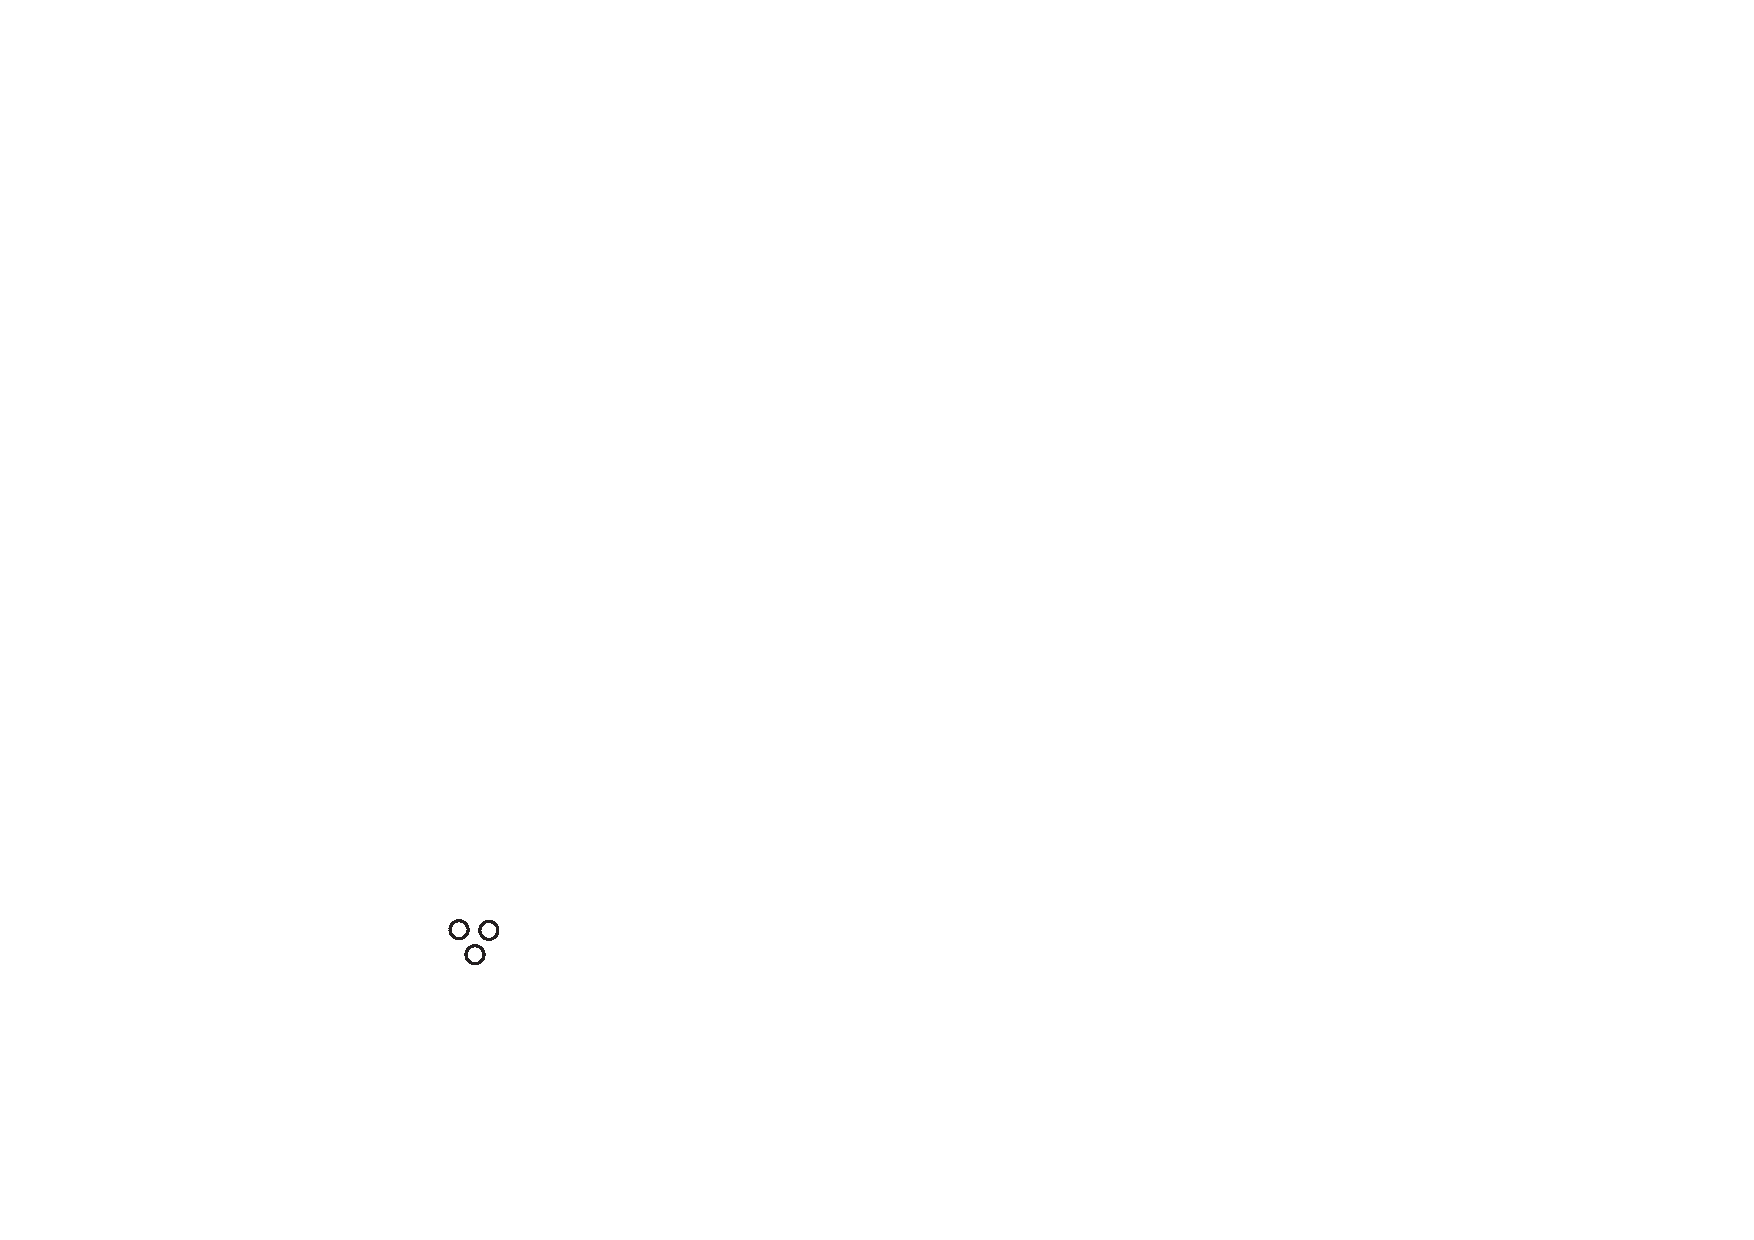
\includegraphics[width=0.02\textwidth]{images/sym-oleum2.pdf} \protect
\includegraphics[width=0.02\textwidth]{images/vitriol.pdf}\textsuperscript{li}\\%
S.~560, Z.~9 & \textit{statt} In \protect
\includegraphics[width=0.02\textwidth]{images/vitriol.pdf}\textsuperscript{li} \textit{lies} In \protect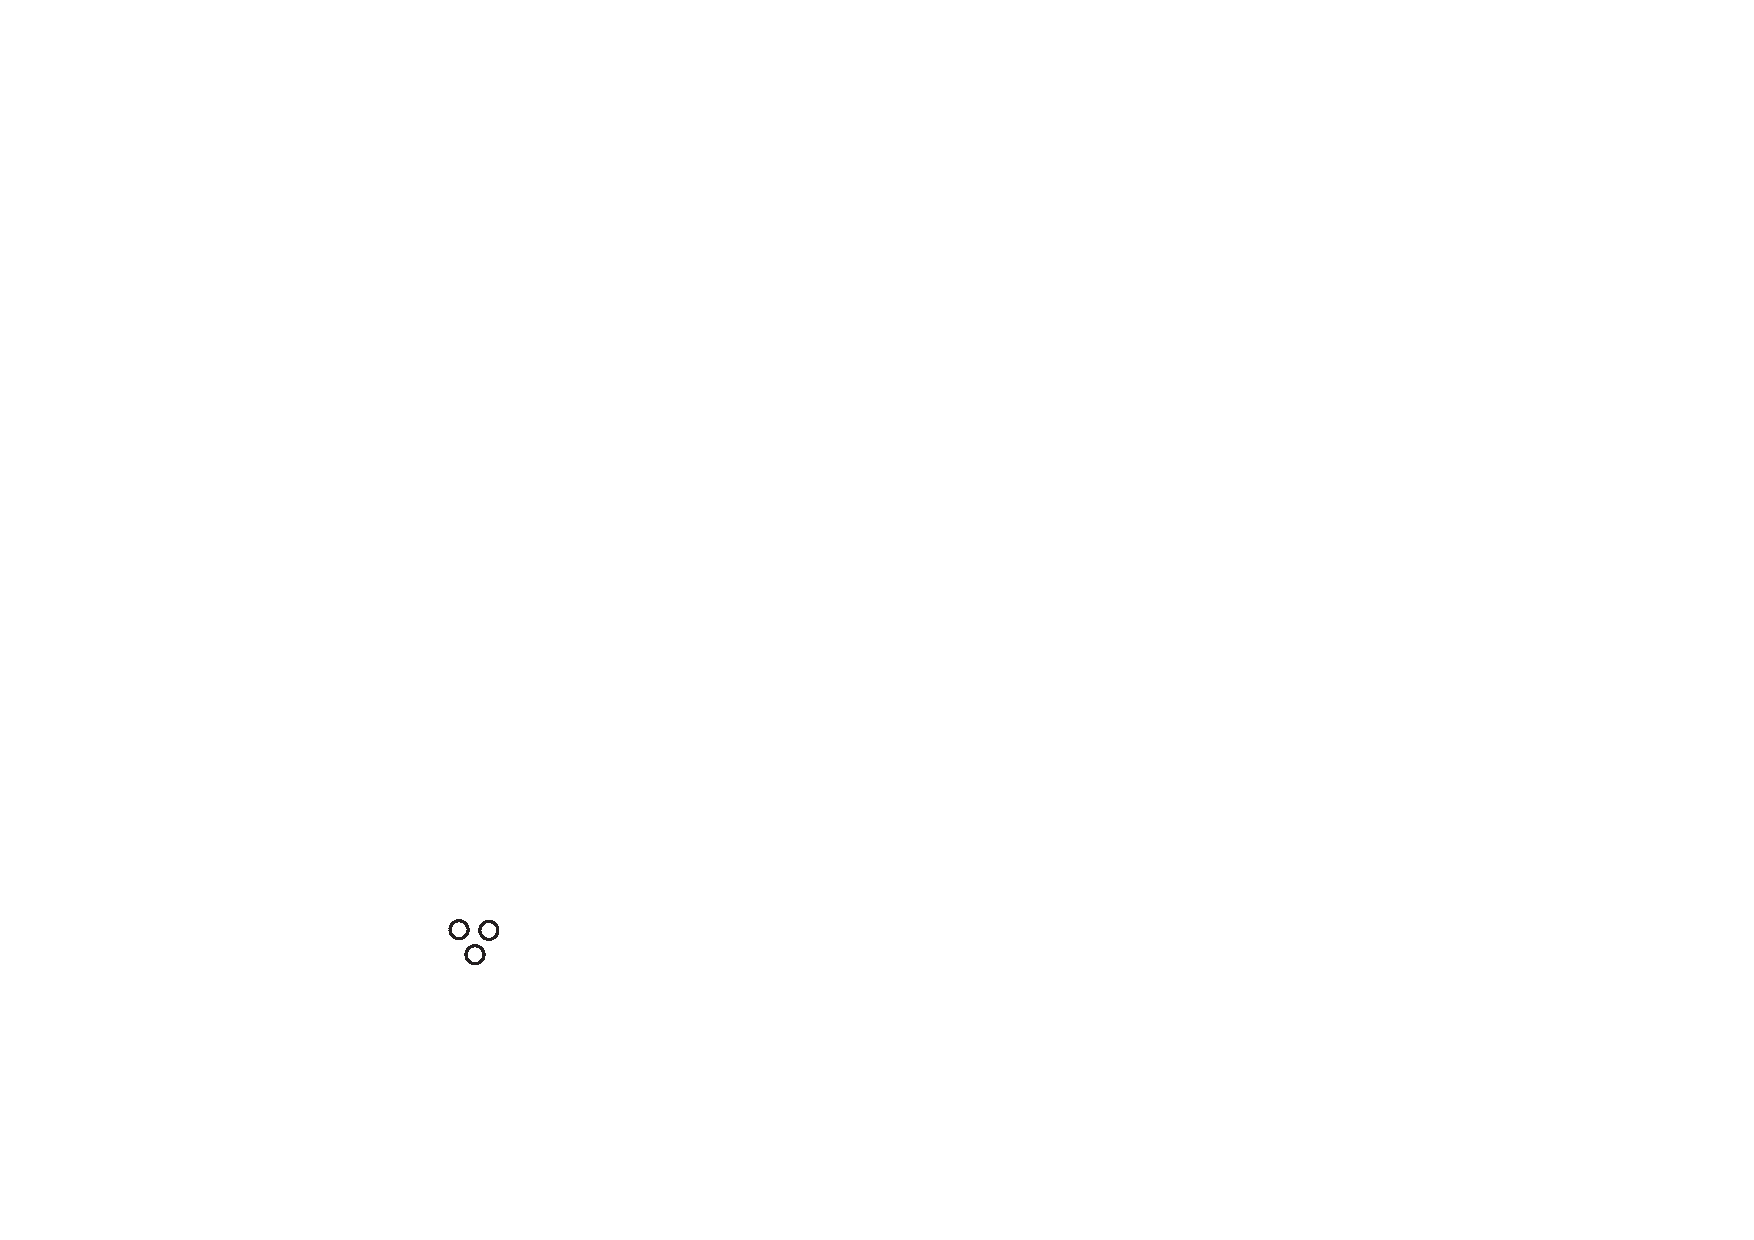
\includegraphics[width=0.02\textwidth]{images/sym-oleum2.pdf} \protect
\includegraphics[width=0.02\textwidth]{images/vitriol.pdf}\textsuperscript{li}\\%
S.~580, Z.~16 & \textit{statt} couleurs couleur, \textit{lies} couleurs,\\%
S.~581, Z.~2 & \textit{statt} 4\textsuperscript{o} \textit{lies} 8\textsuperscript{o}\\%
S.~587, Z.~2 & \textit{statt} Bl.~87~r\textsuperscript{o}. \textit{lies} Bl.~87.\\%
S.~644, SV Nr.~25 & \textit{statt} \textsc{Baliani, G.} \textit{lies} \textsc{Baliani, G.\,B.}\\%
S.~644, SV Nr.~25 & \textit{statt} \textit{fluidorum et solidorum.} \textit{lies} \textit{solidorum et liquidorum.}\\%
S.~647, SV Nr.~69 & \textit{statt} \textit{Pereiesc} \textit{lies} \textit{Peiresc}\\%
S.~653, SV Nr.~164 & \textit{statt} 1664. \textit{lies} 1661.\\%
\end{longtable}
%%
\vspace*{1.0ex}% PR: Rein provisorisch!
%%
\newpage
\noindent%
Zu Band VIII, 2:\\% [1.0ex]
%%
\setlength\LTleft{0pt}\setlength\LTright{0pt}
\begin{longtable}{lp{100mm}}
\footnotesize
S.~126, Marg. zu Z.~8 & \textit{ergänze Erl. zu} Ellipticus Compassus forma crucis: Siehe \cite{?????}\textsc{A. von Braunmühl}, \glqq Historische Studie über die organische Erzeugung ebener Curven von den ältesten Zeiten bis zum Ende des achtzehnten Jahrhunderts\grqq, in \textsc{W. Dyck} (Hrsg.), \textit{Katalog mathematischer und mathematisch-physikalischer Modelle, Apparate und Instrumente}, München 1892, S.~54-88, bes. S.~58 (Proklos), S.~68-70 (Frans van Schooten) und S.~70f. (Apollonius Cattus).\\%
S.~127, Z.~17f. & \textit{ergänze Erl.} \cite{00135}\textsc{M. Thévenot}, \glqq Machine nouvelle pour la conduite des eaux, pour les bâtimens, pour la navigation et pour la pluspart des autres arts\grqq, \textit{JS}, 15. November 1666, S.~439-443. Siehe \textit{LSB} VIII, 1 N.~11, S.~103, Z.~3, Erl.\\%
% S.~128, Erl. zu Z.~1 & \textit{statt} Brief an [...] S.~18-21. \textit{lies} \cite{00135}\glqq Machine nouvelle pour la conduite des eaux, pour les bâtimens, pour la navigation et pour la pluspart des autres arts\grqq, \textit{JS}, 15. November 1666, S.~439-443. Siehe \textit{LSB} VIII, 1 N.~11, S.~103, Z.~3, Erl.\\%
\end{longtable}